\documentclass[letterpaper]{article}

%% Language and font encodings
\usepackage[english]{babel}
\usepackage[utf8x]{inputenc}
\usepackage[T1]{fontenc}

%% Sets page size and margins
\usepackage[letterpaper,top=3cm,bottom=2cm,left=2cm,right=2cm,marginparwidth=1.75cm]{geometry}

%% Useful packages
\usepackage{amsmath}
\usepackage{graphicx}
\usepackage[colorinlistoftodos]{todonotes}
\usepackage[colorlinks=true, allcolors=blue]{hyperref}
\usepackage{mathtools}
\usepackage{latexsym}
\usepackage[cache=false]{minted}
\usepackage{xcolor}

\definecolor{LightGray}{gray}{0.9}
%\definecolor{DarkGray}{gray}{0.1}

%\pagecolor{DarkGray}

\usemintedstyle{borland}

%New colors defined below
\definecolor{codegreen}{rgb}{0,0.6,0}
\definecolor{codegray}{rgb}{0.5,0.5,0.5}
\definecolor{codepurple}{rgb}{0.58,0,0.82}
\definecolor{backcolour}{rgb}{0.95,0.95,0.92}

\title{Speech Processing Final Project}
\author{Matt Ruffner, Charles Vanderpool}

\begin{document}
\maketitle

\section{Overview}

This project aims to implement a rudimentary PA system that will take an input signal from a microphone, encode the speech using a Code Excited Linear Prediction (CELP) based coding scheme, transmit the encoded signal over a serial connection, then decode and play the speech signal on a speaker. In order to implement such a system, the use of two libraries: the Audio library and the Speex Codec library. The Audio library provides simple audio input and playback capabilities and the Speex Codec implements the CELP based encoder and decoder. The system will be implemented on one Arduino Teensy 3.6 development board connected to a speaker. The hardware setup is shown in Figure \ref{hardware}.

\begin{figure}[h!]
    \centering
    \includegraphics[width=10cm]{hard}
    \caption{Hardware Diagram}
    \label{hardware}
\end{figure}


CELP is based on the source-filter model of speech production, a model that assumes that the vocal chords are the source of an excitation signal that is filtered by the vocal tract to shape the spectrum of speech. Using linear prediction(LP), a model is obtained that can be encoded then transmitted or stored with a smaller memory footprint than the speech signal itself. The linear prediction coefficients are typically found using the Levinson-Durbin algorithm. These coefficients are then used as the poles of an IIR filter to obtain the excitation sequence. In CELP coding, the excitation sequence is then used estimate the pitch of the speech signal. This is done by simply multiplying a previous period of the excitation signal $e[n]$ by a pitch gain factor $\beta$ shown in Equation \ref{pitchpred},

\begin{equation}\label{pitchpred}
    e[n] \simeq p[n] = \beta e[n-T]
\end{equation}
where T is the pitch period and $T >> N$. For each sub-frame of the speech frame, a code-book of stochastic signals~\cite{KimY.E2001Ecdf} is searched using analysis by synthesis to perceptually optimize the decoded speech signal. The encoded signal is transmitted as a series of code-words from the code-book, the pitch prediction, and the vocal tract reflection coefficients.

To decode the signal, the pitch prediction and the code-word sequence are summed as shown in Equation \ref{excite} to reconstruct the excitation signal,

\begin{equation}\label{excite}
    e[n] \simeq p[n] + c[n] = \beta e[n-T] +c[n]
\end{equation}
where c[n] is the sequence of code-words. This process is shown in the z-domain in Equation \ref{exitetranfunc}.

\begin{equation}\label{exitetranfunc}
    X(z) = \frac{C(z)}{A(z)(1-\beta z^{-1})}
\end{equation}
Finally, the excitation signal is filtered using the vocal tract reflection coefficients to synthesize the speech signal.

\section{Approach}

The system first collect data from an analog to digital converter instantiated by the Audio library. In order to access the data collected by the \texttt{AudioStream} class, a new class must be defined that inherits the \texttt{AudioStream} class~\cite{audio}. This new class, named \texttt{CELPEncoder}/\texttt{CELPDecoder} in the respective Arduino sketches, must define a function called update. This function is called by the \texttt{AudioStream} class every 2.9 ms using an interrupt service routine. Each time the function is called, 128 samples quantized to 16 bit integers are collected from the ADC and stored in an array. This data is then passed to the Speex CELP encoder. After the signal is encoded, it is transmitted to the decoder board through a serial port.

On the decoder board, a very similar process takes place, except the CELP data is decoded, then passed to the update function to be  sent to the digital to analog converter(DAC). Figure \ref{Software} show show the software flowcharts for the encoder and decoder respectively. The most relevant source code is provided in the appendix, and the full source code is available at \url{http://github.com/ruffner/celp-pa}.

\begin{figure}[h!]
    \centering
    \includegraphics[width=10cm]{soft}
    \caption{Software Flowchart}
    \label{Software}
\end{figure}

To implement a CELP based encoder/decoder on an Arduino Teensy3.2, the Speex Codec API was integrated into the project implementation in narrow-band mode. The speech signal, sampled at 8 kHz, is broken into 20 ms (160 samples) frames that are divided into 4 sub-frames of 40 samples each~\cite{valin2007speex}. The line spectral pairs(LSP), a representation of LPC coefficients that are quantization safe, are encoded at the frame level as well as the global excitation gain GFRAME. In the decoder, the LSP coefficients are converted back to LPC coefficients. 

The adaptive code book for Speex is generated using an integer to encode the pitch period and a 3-tap predictor as shown in Equation \ref{exitsynth}, 

\begin{equation}\label{exitsynth}
    e_a[n] = g_0e[n-T-1] + g_1e[n-T] + g_2e[n-T+1] 
\end{equation}

where G0, G1, and G2 are the quantized pitch gains and $e[n]$ is the codec excitation memory~\cite{valin2007speex}. When the pitch period is smaller than the sub-frame size, the excitation is repeated at a period T. Each sub-frame is encoded using an analysis-by-synthesis closed loop optimizer shown in Figure \ref{loopopt}. this optimization loop generates the adaptive codebook and the sub-frame gain. Figure \ref{abs} shows the process by which the LSPs and the frame gain are generated and vector quantized.

\begin{figure}[h!]
    \centering
    \includegraphics[width=10cm]{closed}
    \caption{Closed-loop Sub-frame Analysis-by-synthesis~\cite{valin2007speex}}
    \label{loopopt}
\end{figure}

\begin{figure}[h!]
    \centering
    \includegraphics[width=10cm]{abs}
    \caption{Open-loop Frame Analysis~\cite{valin2007speex}.}
    \label{abs}
\end{figure}

The Speex code is decoded using the same process detailed by Equations 1-3. The only difference in the decoder is that the synthesis filter that acts as the vocal tract is modeled using an enhanced filter~\cite{valin2007speex} with the transfer function given in Equation \ref{synthtran}.

\begin{equation}\label{synthtran}
    S^\prime(z) = \frac{A(z/a_2)A(z/a_3)}{A(z)A(z/a_1)}
\end{equation}
where $a_1$ and $a_2$ depend on the quality mode and

\begin{equation}\label{supp}
    a_3 = \frac{1}{r}\left(1-\frac{1-ra_1}{1-ra_2}\right)
\end{equation}
where $r = 0.9$.

Figure \ref{bitalloctab} shows the bit allocation scheme for each Speex mode of operation. The mode used in this project is mode 3, allowing for a bit rate of 8 kbps as shown in Fig. \ref{qualtab}. It is expected that there will some noticeable artifacts or noise introduced through the encode/decode process.

\begin{figure}[h!]
    \centering
    \includegraphics[width=12cm]{bitalloctable}
    \caption{Speex Mode and Bit-rate~\cite{valin2007speex}}
    \label{bitalloctab}
\end{figure}

\begin{figure}[h!]
    \centering
    \includegraphics[width=12cm]{qualitytable}
    \caption{Speex Mode and Quality~\cite{valin2007speex}}
    \label{qualtab}
\end{figure}

\newpage

\section{Limitations}

The limiting factors in this project stem from both the hardware used and the libraries chosen. Originally, the goal was to implement the encoder and decoder of separate Arduino boards that communicate using RFM95 radio transmitters. However, the transmitters only sent 2 sets of CELP data before the program crashed. after a considerable amount of time was spent trying to debug this issue, the decision was made to write the encoder and decoder on the same board in order to focus on implementing the CELP based coding scheme.

Another limitation to the implementation is the nature of the Audio library. Because the \texttt{AudioStream} class calls an interrupt service routine every 2.9 milliseconds with a variable amount of processing to complete. The non-constant interruption of the process causes a clicking artifact to be heard in the output to the speaker. In addition to this artifact, the functions used to up-sample and down-sample the signal are flawed and cause the speech output to be unintelligible.

Finally, there are some limitation that come from the Speex library itself. The Speex documentation states that there have been no Mean Opinion Score testing done on the quality of the speech synthesis, so the results in Table 2 may not be entirely quantitative. Additionally, the Speex library is very susceptible to error when a delay is introduced between the data capture and playback. This property is the likely root of the clicking artifacts and the lack of intelligible speech in the output signal.

\section{Results}

The first success of this project was getting the Speex library ported to the Arduino environment, which took much work in header editing and file reorganization since the include paths in the Arduino environment are ridiculous. Once this was achieved, focus on implementing Speex functionality started.

After initially trying to incorporate two micro-controllers and radio modules into this project, we eventually decided to use serial communication to send the encoded CELP data between micro-controllers. This, however, proved to be a larger amount of complexity than was appropriate for the scope of this project and contributed to excessive delay between the data input and output.

As a test, a sine wave was generated as the input signal and changed from 220Hz to 880Hz every second. There are audible differences in the output sound from the speaker when this input mode is selected. To test the intelligibility of speech waveforms and the compression achieved therein, an SD card was used to load in a 16bit PCM WAV file containing a sample from the TIMIT dataset~\cite{timit}.

Since the encoder object outputs a specific number of  bytes per encoding operation, the main loop of the main Arduino sketch file is able to monitor the throughput of the Speex implementation. By measuring the number of bits that are passed between the encoder and decoder every second, the final bit-rate we were able to achieve was $9.351$ kbps. The final system implementation can be seen in Fig. \ref{fig:imp}.


\begin{figure}[h!]
    \centering
    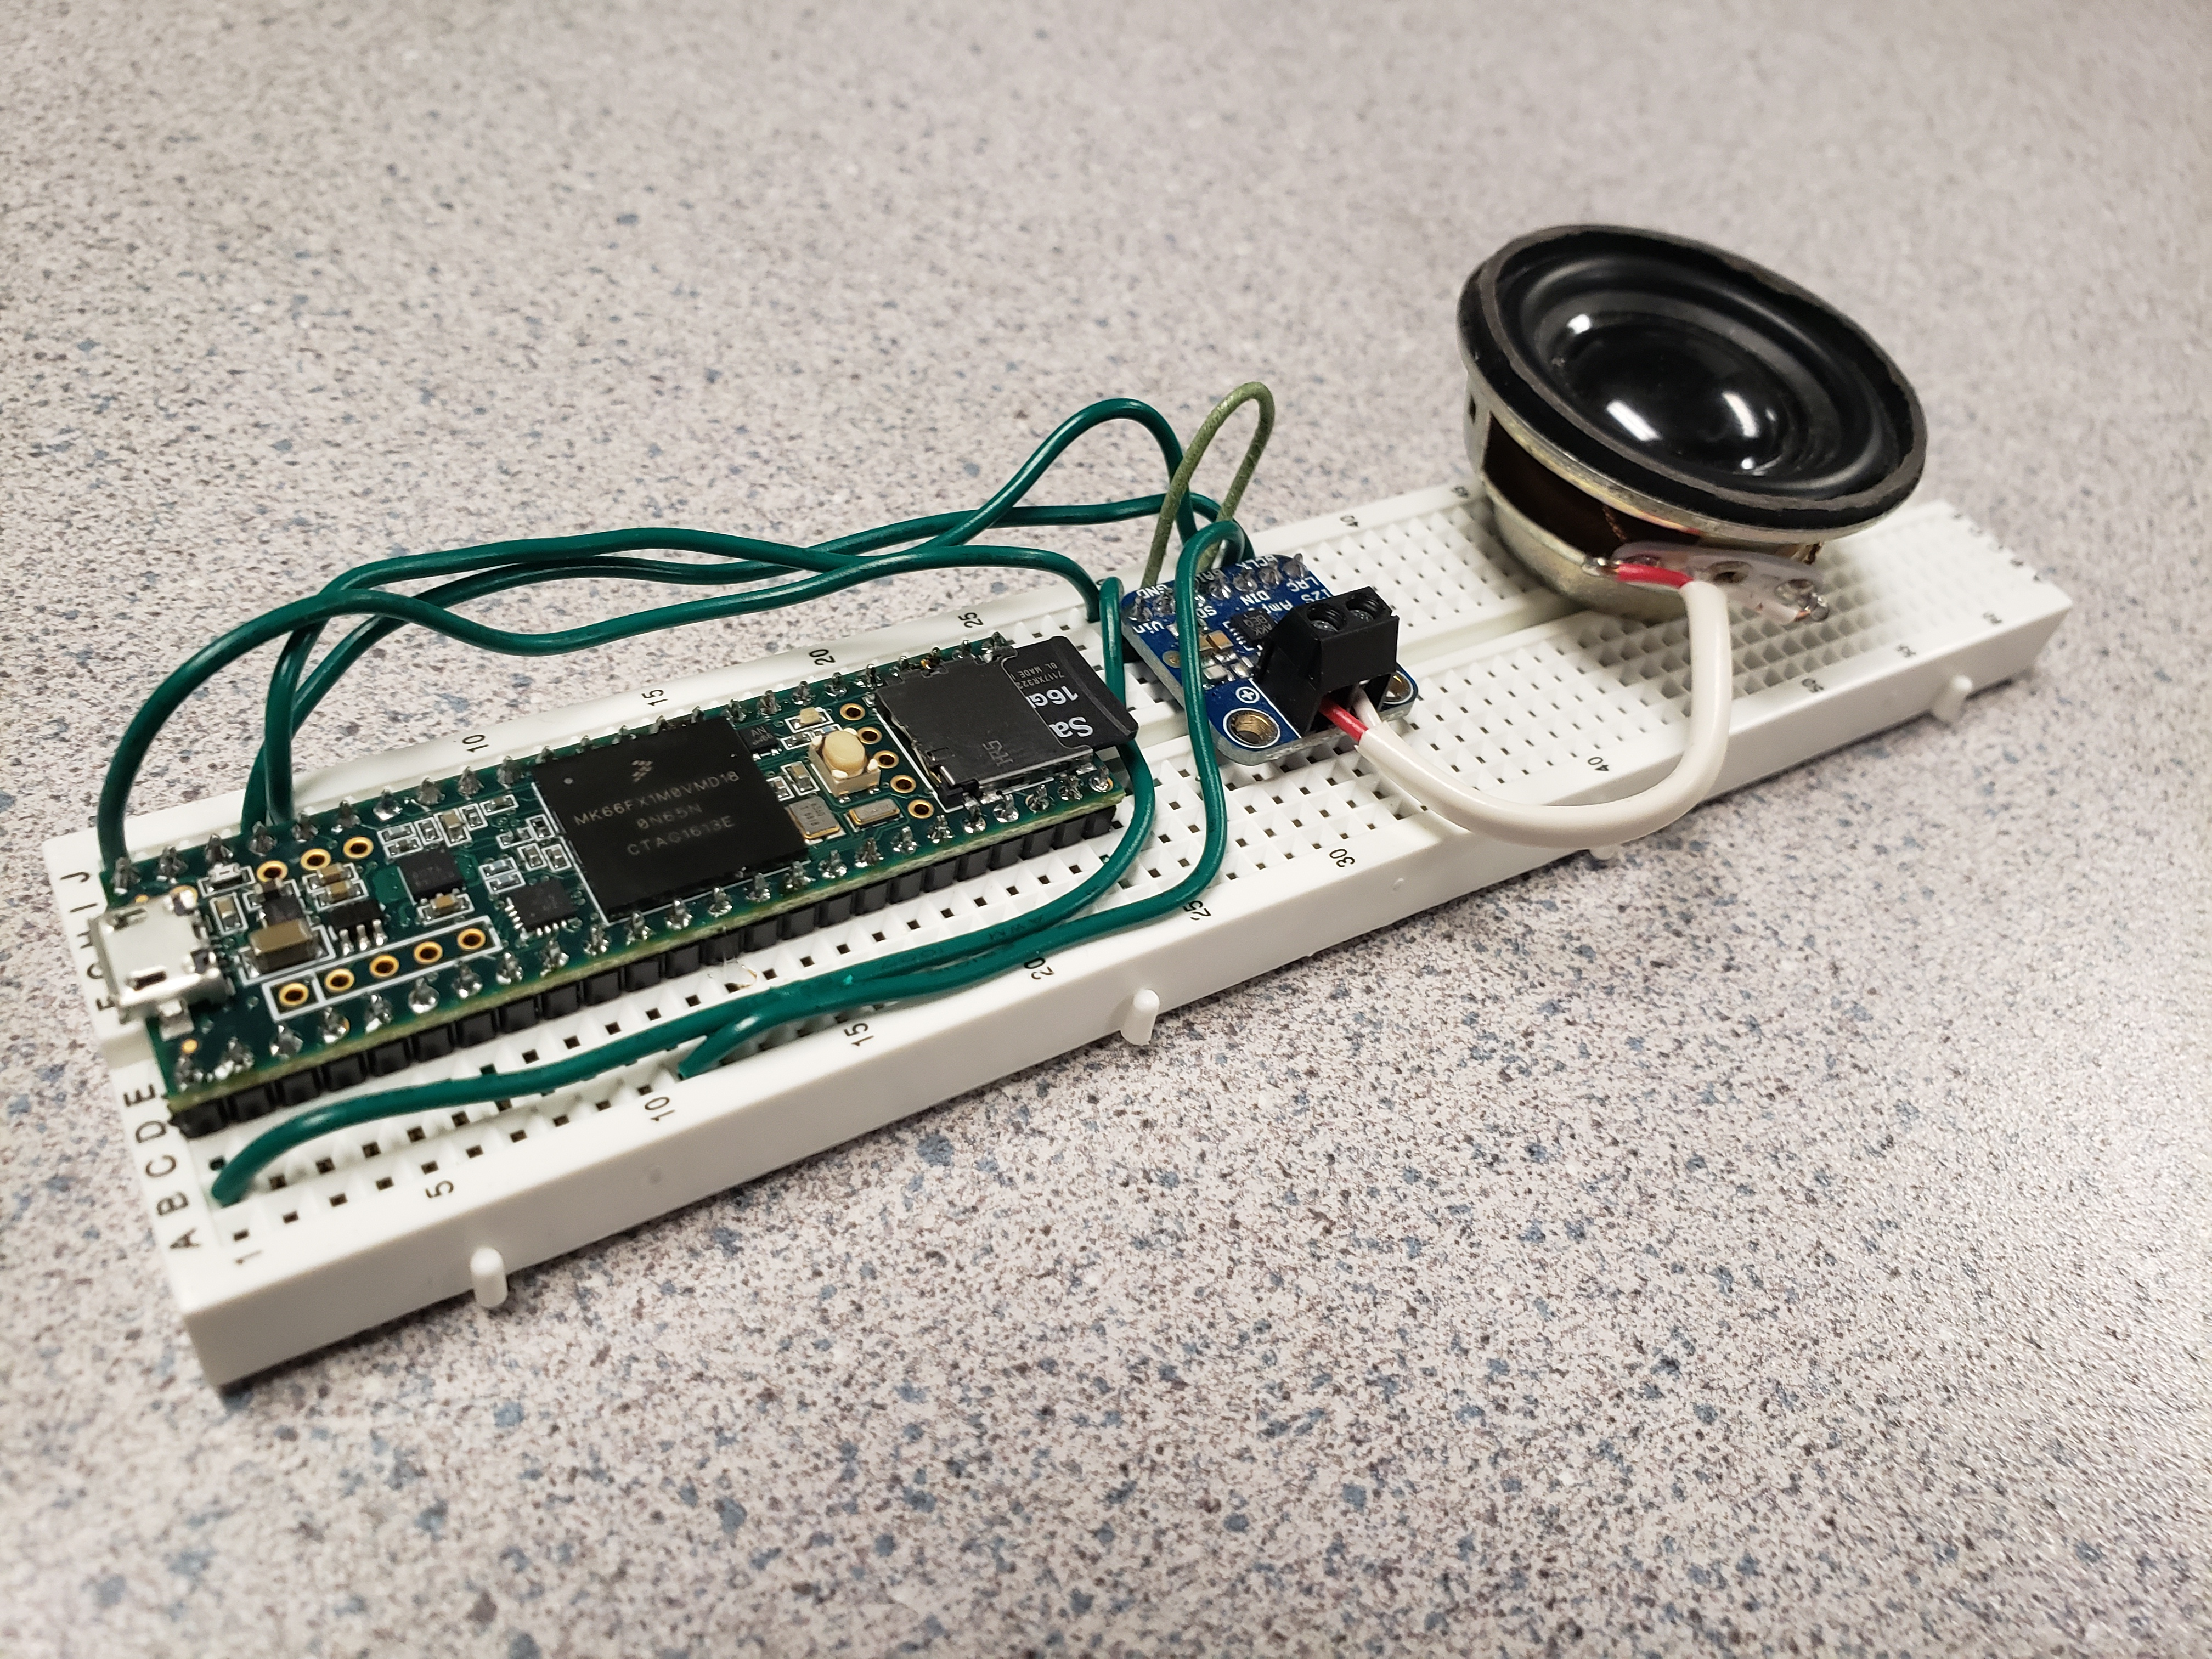
\includegraphics[width=8cm]{speex-system}
    \caption{Final implementation on Teensy 3.6 microcontroller.}
    \label{fig:imp}
\end{figure}

\newpage

\appendix
\section{\texttt{AudioEffectDownsample.h}}
\begin{verbatim}
#ifndef audio_downsample
#define audio_downsample

#include "Arduino.h"
#include "AudioStream.h"

class AudioEffectDownsample : public AudioStream
{
public:
	AudioEffectDownsample() : AudioStream(1, inputQueueArray),outCount(0),outPos(0) {};
	virtual void update(void);
	int getOutCount();
private:
	int outCount;
  int outPos;
  uint16_t outputBuffer[2*AUDIO_BLOCK_SAMPLES];
	audio_block_t *inputQueueArray[1];
};

#endif
\end{verbatim}

\section{\texttt{AudioEffectDownsample.cpp}}
\begin{verbatim}
#include "effect_downsample.h"

int AudioEffectDownsample::getOutCount()
{
	return outCount;
}

void AudioEffectDownsample::update()
{
	audio_block_t *inBlock, *outBlock;
	uint16_t *inData, *outData;
	
	// try to receive 44.1kHz audio data and allocate output block
	inBlock =  receiveReadOnly(0);
	outBlock = allocate();
	if (inBlock == NULL) {
		// no input data, cant update
		return;
	}
	if (outBlock == NULL) {
		// no more audiomemory
		return;
	}
	
	// cast data to unsigned 16 bit ints
	inData = (uint16_t *)inBlock->data;
	outData = (uint16_t *)outBlock->data;

  
  if( outPos < AUDIO_BLOCK_SAMPLES ){   
    // fill in outputBuffer with incoming data
    int inPos = 0;
    while( inPos < AUDIO_BLOCK_SAMPLES ){
      outputBuffer[outPos] = inData[inPos];
      inPos = inPos + 5;
      outPos++;
    }
  }
  if( outPos >= AUDIO_BLOCK_SAMPLES ){
    // have enough samples to transmit, copy to out buffer and transmit
    for( int i=0; i<AUDIO_BLOCK_SAMPLES; i++ ){
      outData[i] = outputBuffer[i];
    }
    outPos -= AUDIO_BLOCK_SAMPLES;

    transmit(outBlock);
  }
	
	release(inBlock);
  release(outBlock);
}
\end{verbatim}

\section{\texttt{CELPEncode.h}}
\begin{verbatim}
#ifndef celp_encode_h
#define celp_encode_h

#include "Arduino.h"
#include "AudioStream.h"
#include "speex.h"

#define FRAME_SIZE 160

class CELPEncode : public AudioStream 
{
public:
  CELPEncode() : AudioStream(1, inputQueueArray),act(false),dataReady(false),nbytes(0), curSamples(0) {};
  ~CELPEncode() {
	  speex_encoder_destroy(speexState);
	  speex_bits_destroy(&speexBits);
  }
  virtual void update(void);
  int init();
  bool available();
  int getNumBytes();
  uint8_t *getDataPointer();
  
private:
  static void *speexState;
  static SpeexBits speexBits;
  char cbits[200];
  bool act = false;
  int curSamples;
  uint16_t sampleBuffer[FRAME_SIZE];
  int nbytes;
  volatile bool dataReady = false;
  audio_block_t *inputQueueArray[1];
};

#endif

\end{verbatim}

\section{\texttt{CELPEncode.cpp}}
\begin{verbatim}
#include "CELPEncode.h"

void * CELPEncode::speexState;
SpeexBits CELPEncode::speexBits;

int CELPEncode::init()
{
  if( act ) return -2;
    
  // create a new narrowband encoder
  speexState = speex_encoder_init(&speex_nb_mode);
  
  // set the encoder quality
  int temp=4;
  int result = speex_encoder_ctl(speexState, SPEEX_SET_QUALITY, &temp);
  
  
  // initialization of speex bits structure
  speex_bits_init(&speexBits);

  // indicate that init() has been called
  act = true;
  
  return result; 
}

bool CELPEncode::available()
{
  return dataReady;
}

int CELPEncode::getNumBytes()
{
  return nbytes;
}

uint8_t *CELPEncode::getDataPointer()
{
	dataReady = false;
	return (uint8_t *)cbits;
}

void CELPEncode::update()
{
  audio_block_t *inBlock;
  uint16_t *inData;
  int inSamples;

  // return if begin() has not been called
  if (!act) return;

  // try receive new audio data and allocate output block
  inBlock =  receiveReadOnly(0);

  if (inBlock == NULL) {
    // no input data, cant update
    return;
  }
  
	// receive data downsampled to roughly 8kHz from 
	// the 44.1kHz that the audio library creates
	inData = (uint16_t *)inBlock->data;

	// how many samples did we receive
  inSamples = AUDIO_BLOCK_SAMPLES;
  
  // if we need to just buffer up data to fill a frame for speex computation
  if( curSamples+inSamples < FRAME_SIZE ){
	  
	  // append input data to our sampleBuffer
	  for( int i=curSamples; i<curSamples+inSamples; i++ ){
		  
		  // +1 offset to account for the first position storing the number of samples 
		  sampleBuffer[i] = inData[i-curSamples+1];
	  }
	  curSamples += inSamples;
  } 
  // otherwise we are receiving enough to fill a frame, possibly more
  else {
	  
	  // append enough of the input data to our sample buffer to fill it
	  for( int i=curSamples; i<FRAME_SIZE; i++ ){
		  
		  // +1 offset to account for the first position storing the number of samples 
		  sampleBuffer[i] = inData[i-curSamples+1];
	  }
	  
	  // now our sample buffer is full, so process it
	  speex_bits_reset(&speexBits);
	  speex_encode_int(speexState, (spx_int16_t*)sampleBuffer, &speexBits);
	  nbytes = speex_bits_write(&speexBits, cbits, 200);
	  dataReady = true;
	  
	  // fill the beginning of the sample buffer with the excess input data
	  int offset = FRAME_SIZE-curSamples;
	  for( int i=0; i<inSamples-offset; i++ ){
		  
		  // +1 offset to account for the first position storing the number of samples 
		  sampleBuffer[i] = inData[offset+i+1];
	  }
	  curSamples = inSamples-offset;
	  dataReady = true;
  }

  release(inBlock);
}
\end{verbatim}

\section{\texttt{CELPDecode.h}}
\begin{verbatim}
#ifndef celp_decode
#define celp_decode

#include "Arduino.h"
#include "AudioStream.h"
#include "speex.h"

#define FRAME_SIZE 160

class CELPDecode : public AudioStream
{
public:

	// Constructor
	CELPDecode() : AudioStream(0, NULL),act(false),hasProcessed(true),inputBytes(0),outPos(0),tempPos(0) {};
	
	// Deconstructor
	~CELPDecode(void) {
		speex_bits_destroy(&bits);
		speex_decoder_destroy(dec_state);
	}
	
	// called first to initialize class
	int init(void);
	
	// pass data to buf from outside class, do be decoded
	void feed(char* buf, int len);

	
	// return if the update function has processed the input data supplied with feed()
	// indicating the decoder is ready to be fed more data
	bool consumed(void);
	
	//update called by Audio Library
	virtual void update(void);
	
private:
	
	//speex vars
	SpeexBits bits;
	void *dec_state;
		
	//speex input set by feed
	char input[FRAME_SIZE];
	int inputBytes;	

	// since this size is larger than audio_block_samples, will have to transmit in chunks
	uint16_t outBuffer[FRAME_SIZE];
	uint16_t tempBuffer[FRAME_SIZE];
	int outPos, tempPos;
	
	// initialization and decode state vars
	bool act, hasProcessed;
};
\end{verbatim}


\section{\texttt{CELPDecode.cpp}}
\begin{verbatim}
#include "CELPdecode.h"

// called first - initialized speex decoder
int CELPDecode::init(void)
{
	if( act ) return -2;
   /*Create a new decoder state in narrowband mode*/
   dec_state = speex_decoder_init(&speex_nb_mode);

   /*Set the perceptual enhancement on*/
   int tmp=1;
   int result = speex_decoder_ctl(dec_state, SPEEX_SET_ENH, &tmp);

   /*Initialization of the structure that holds the bits*/
   speex_bits_init(&bits);
   
   act = true;
   
   return result;
}

//set_buf populates buf frorm bufin to be used in the deocde process
void CELPDecode::feed(char* bufin, int len)
{
	for(int i = 0; i<len; i++){
		input[i] = bufin[i];
	}
	inputBytes = len;
	hasProcessed = false;
}

// returns true when data supplied with feed() has been processed, indicating more data
// is ready to be fed
bool CELPDecode::consumed()
{
	return hasProcessed;
}

//update is run every 2.9 ms or so. this will read allocate a sound 
//block, decode the CELP data, the transmit the reult to the DAC
void CELPDecode::update(void)
{
	audio_block_t *outBlock;
  uint16_t *outData;
	outBlock = allocate();

	// no where to store output data
	if(outBlock == NULL) return;
	
	outData = (uint16_t*)(outBlock->data);

	// dont run if not initialized
	if( !act ) return;

	// if we have new data to process, do it
	if( !hasProcessed && inputBytes){
	
		// read input bytes to speex bits struct
		speex_bits_read_from(&bits, input, inputBytes);

		// decode speex bits struct
		speex_decode_int(dec_state, &bits, (spx_int16_t *)outBuffer);
		
		hasProcessed = true;
	}
		
	// if we have remaining data, fill output block with combination of old and new data
	if( tempPos ) {
		// we have old data that needs to be filled in first
		for( int i=0; i<tempPos; i++ ){
			outData[i] = tempBuffer[i];
		}
		outPos = tempPos;
		
		// now fill in remaining space in outData with freshly decoded data
		for( int i=outPos; i<AUDIO_BLOCK_SAMPLES; i++ ){
			outData[i] = outBuffer[i-outPos];
		}
		
		// now store the rest of the newly decoded data into tempBuffer
		tempPos = AUDIO_BLOCK_SAMPLES-outPos;
		for( int i=tempPos; i<FRAME_SIZE; i++ ){
			tempBuffer[i-tempPos] = outBuffer[i];
		}
	} 
	// otherwise just copy in the initial data 
	else {
		// fill output block with initial data
		for( int i=0; i<AUDIO_BLOCK_SAMPLES; i++ ){
			outData[i] = outBuffer[i];
		}
		
		// now store the rest of the newly decoded data into tempBuffer
		tempPos = AUDIO_BLOCK_SAMPLES;
		for( int i=tempPos; i<FRAME_SIZE; i++ ){
			tempBuffer[i-tempPos] = outBuffer[i];
		}
	}
	
	transmit(outBlock);
	release(outBlock);
}
\end{verbatim}

\section{\texttt{AudioEffectUpsample.h}}
\begin{verbatim}
#ifndef audio_upsample
#define audio_upsample

#include "Arduino.h"
#include "AudioStream.h"

class AudioEffectUpsample : public AudioStream
{
public:
	AudioEffectUpsample() : AudioStream(1, inputQueueArray),rxCount(0) {};
	void init(void);
	virtual void update(void);
private:
	int rxCount;
	int txPos;
	uint16_t inputBuffer[7][AUDIO_BLOCK_SAMPLES];
	uint16_t outputBuffer[6][AUDIO_BLOCK_SAMPLES];
	audio_block_t *inputQueueArray[1];
};

#endif
\end{verbatim}


\section{\texttt{AudioEffectUpsample.cpp}}
\begin{verbatim}
#include "effect_upsample.h"

void AudioEffectUpsample::update()
{
	audio_block_t *inBlock, *outBlock;
	uint16_t *inData, *outData;
	bool flag = false;
	int i, inSamples;
	
	// allocate output
	outBlock = allocate();
	
	// see if there is 8kHz data ready, this will not be the case every time
	inBlock =  receiveReadOnly(0);
	
	// if outblock is null we can't do anything
	if (outBlock == NULL) {
		// no more audiomemory
		return;
	}  else {
		outData = (uint16_t *)outBlock->data;
	}
	
	// if inblock isnt null we can upsample the incoming data
	if (inBlock != NULL) {
		// upsample and buffer the new input data
		
		// cast data to unsigned 16 bit ints
		inData = (uint16_t *)inBlock->data;
				
		// 128 samples at 8kHz = ~706 samples at 44.1kHz
		// so need 6 audio blocks to store the upsampled data
		int inPos = 0;
		bool flag = false;
		
		// iterate through output blocks
		for( int i=0; i<6; i++ ){
			
			for( int j=0; j<AUDIO_BLOCK_SAMPLES; j++ ){
				
				outputBuffer[i][j] = inData[inPos];
				
				if( (j+1) % (flag?6:5)==0 ){
					inPos++;
          if( inPos >= AUDIO_BLOCK_SAMPLES ){
            inPos = 0;
            txPos = 0;
            break;
          }
					flag=!flag;
				}
				
				
			}
			
		}
	}
	// transmit buffered upsampled data
  // if we are starved for data, resend last chunk
  if( txPos > 5 ){
    txPos = 5;
  }
  for( int i=0; i<AUDIO_BLOCK_SAMPLES; i++ ){
    outData[i] = outputBuffer[txPos][i];
  }
  txPos++;

	// outBlock now has fewer samples than inblock, so 
	transmit(outBlock);
  release(outBlock);
	release(inBlock);
}
\end{verbatim}
\bibliographystyle{ieeetr}
\bibliography{refs.bib}
\end{document}